\documentclass[10pt,twocolumn]{article}

% ---- arXiv-portable packages (compile under pdflatex and tectonic/XeTeX) ----
\usepackage[margin=0.85in]{geometry}
\usepackage{graphicx}
\usepackage{booktabs}
\usepackage{amsmath}
\usepackage{amssymb}
\usepackage{xcolor}
\usepackage{url}
\usepackage[hidelinks]{hyperref}
% allow long URLs to break at more points (e.g. underscores) so bib entries don't overflow
\Urlmuskip=0mu plus 1mu\relax
\def\UrlBreaks{\do\/\do\-\do\_\do\.\do\a\do\b\do\c\do\d\do\e\do\f\do\g\do\h\do\i\do\j\do\k\do\l\do\m\do\n\do\o\do\p\do\q\do\r\do\s\do\t\do\u\do\v\do\w\do\x\do\y\do\z}
\usepackage{caption}
\captionsetup{font=small,labelfont=bf}

\graphicspath{{figures/}}

% ---- One-line renamable identity ----
\newcommand{\datasetname}{\mbox{CyberKnowledgeSFT}}      
\newcommand{\systemname}{\mbox{AirgapForge}}          
\newcommand{\offensivename}{\mbox{VulnExploit-SFT}}   

\newcommand{\ethicsbox}[1]{\par\medskip\noindent\fbox{\parbox{0.95\columnwidth}{\small #1}}\par\medskip}

\title{The Cheap Path to an Offensive LLM:\\
A Local, Measured Dual-Use Capability Study}

\author{
Tristan J. Pereira\\
Independent Security Researcher\\
tristanjpereira@gmail.com
}
\date{}

% Don't vertically stretch columns to the bottom margin; keep natural
% paragraph spacing and let any slack fall at the column bottom.
\raggedbottom

\begin{document}
\maketitle

\begin{abstract}
Instruction-tuning datasets for cybersecurity have, until recently, been
assembled with the help of commercial, cloud-hosted language models. We ask a
narrower and more uncomfortable question: what happens when the entire
construction and fine-tuning loop is moved onto a single consumer
Apple~Silicon machine, with no external API in the path and no provider side
safety filter shaping the corpus? We describe \systemname, a fully on-device
reimplementation of a published cybersecurity data pipeline built on Apple's
MLX framework. Building on the work of
ElZemity et al.~\cite{cyberllminstruct}, we reproduce a defensive instruction
dataset locally and characterize a second, offensive branch that
removes the pipeline's safety-alignment stage and trains models, including
\emph{abliterated} (safety-stripped) bases, to produce exploitation guidance
for vulnerable code. We then measure a full matrix of alignment (aligned vs.\
abliterated) $\times$ fine-tuning (base vs.\ offensively fine-tuned) across
three open model families on capability, safety, and audit quality. The results
are stark: abliteration removes refusals at almost no capability cost, and
offensive fine-tuning drives refusal to zero and attack success rate to
$96$--$100\%$ on \emph{every} base, including those that still refused a fifth
of requests while aligned. The whole procedure runs on a single desktop at no
marginal cost: a complete fine-tune takes hours, not a cloud budget.  We do
\emph{not} release exploitation payloads, offensive weights, the dataset, or the
raw generations: only aggregate metrics. Our contribution is a warning made
concrete and measured: the barrier to a locally hosted, uncensored,
exploitation capable LLM is now a weekend of compute on hardware
that fits under a desk.
\end{abstract}

\section{Introduction}

Fine-tuning large language models (LLMs) on cybersecurity data is a
double-edged experiment. The same instruction data that teaches a model to
explain a CVE, triage an advisory, or reason about an attack technique also
moves the model toward producing operational offensive content, up to agents
that autonomously exploit real vulnerabilities~\cite{fang2024exploit}. That
fine-tuning can \emph{degrade} a model's safety is by now well
documented~\cite{qi2023finetuning,lermen2023lora}; ElZemity et
al.~\cite{cyberllminstruct} made the cybersecurity case concrete with
CyberLLMInstruct.

That study, like most dataset construction efforts, relied on commercial,
cloud-hosted models to filter and synthesize data. This paper examines what
changes when the cloud is removed from the loop entirely. We take the
CyberLLMInstruct pipeline as our starting point and re-engineer its
LLM dependent stages to run fully on-device using Apple's MLX
framework~\cite{mlx}, then fine-tune a range of open models locally with
low-rank adaptation~\cite{lora}. Two properties of this all local setting
motivate the paper. First, no third-party service ever observes the
security data, and no provider safety filter constrains what the pipeline can
generate, removing both a confidentiality concern and a safety guardrail.
Second, the cost: the hardware is a single desktop, and the models
that make it work, including \emph{abliterated}~\cite{abliteration} variants
with their refusal behavior surgically removed, are freely downloadable - well
within reach with the majoritity of laptops from the last decade.

We deliberately push this to its uncomfortable conclusion. Alongside a 
defensive reproduction of the instruction dataset, we build an
\emph{offensive} branch (\offensivename) that strips the pipeline's
safety-alignment stage and uses an abliterated model to synthesize
exploitation write-ups over a public vulnerable code corpus, then fine-tunes
on the result. Our intent is not to ship an ``AI pentesting bot'' but to
document how cheaply and locally one can be approached, and what that implies.
This concern is not hypothetical for us: the author and other practitioners
have used these locally hosted unrestricted LLMs in confidential
red team engagements, which motivated a systematic measurement of what such
models cost to produce, in capability and in safety. We report that
measurement here; we do not report the engagements, which are confidential.

\section{Background and Related Work}
\label{sec:background}

\paragraph{Cybersecurity instruction datasets.}
CyberLLMInstruct~\cite{cyberllminstruct} is the closest prior work and the
direct antecedent of this paper. It assembles a large pseudo-malicious
instruction data spanning malware analysis, phishing, and vulnerability
tasks, fine-tunes a range of models, and reports the safety/capability
trade off. Our work reproduces the \emph{construction} half of that pipeline in a
fully local setting and re-measures that trade off across an
alignment~$\times$~fine-tuning matrix (\S\ref{sec:eval}), adding an
abliteration axis that CyberLLMInstruct did not test.
Cyber specific evaluation has developed alongside these datasets: CyberMetric~\cite{cybermetric} scores security knowledge, while CyberSecEval~\cite{bhatt2023cyberseceval} measures both vulnerable code generation and compliance with cyber attack requests, the latter close in spirit to the attack success rate we report.

\paragraph{On-device inference and fine-tuning.}
Apple's MLX~\cite{mlx} enables inference and LoRA fine-tuning of quantized
open models directly on Apple~Silicon. Combined with low-rank
adaptation~\cite{lora}, it makes both synthetic data generation and
fine-tuning of $30$B class models feasible on a single machine.

\paragraph{Refusal removal (abliteration).}
``Abliteration''~\cite{abliteration} identifies and ablates the direction in a
model's activation space most associated with refusal, producing an open model
that answers requests it would previously decline. Such models are publicly
distributed. We use one both as a data \emph{generator} (to synthesize
offensive content without refusals) and as a fine-tuning \emph{base}, which
lets us compare capability, safety, and training dynamics across aligned and
de-aligned starting points.

\paragraph{Preference optimization.}
Beyond supervised fine-tuning (SFT), we include direct preference
optimization (DPO)~\cite{dpo} and its reference-free variant
ORPO~\cite{orpo} in the pipeline's recipes, used here in a defensive
configuration.

\paragraph{Safety degradation from fine-tuning.}
Research shows that even benign fine-tuning can erode safety
alignment~\cite{qi2023finetuning}, and that low rank fine-tuning can
\emph{deliberately} undo it for a few hundred dollars~\cite{lermen2023lora}. Our setting is the adversarial extreme of
this research (offensive data on a de-aligned base), and we treat it as a
 characterization rather than a capability demonstration.

\section{The On-Device Pipeline}
\label{sec:pipeline}

\systemname{} transforms raw, authoritative security sources into a validated
instruction-response dataset through a sequence of stages, each writing to its
own directory so the pipeline can be inspected and resumed. Every stage that
requires a language model runs locally via MLX; no external API is called at
any point. Seven stages are implemented in the current codebase.

\begin{enumerate}
  \item \textbf{Collection.} A collector harvests from nine public sources
  (NVD, OpenCVE, MITRE ATT\&CK, CAPEC, Ubuntu and Red~Hat advisories,
  Microsoft advisories, arXiv, and CTF data) via APIs, RSS, and scrapers.
  \item \textbf{Filtering.} A two-pass filter first applies a parallelized,
  rule-based keyword and compound term gate (emitting per-entry provenance),
  then a slower on-device LLM enrichment pass that returns a structured
  \texttt{\{technical\_\allowbreak description, risk\_\allowbreak level,
  affected\_\allowbreak systems, mitigations\}} record.
  \item \textbf{Structuring.} Source-specific builders convert filtered
  entries into instruction--response pairs, each with a domain appropriate
  persona prompt; the stage checkpoints and resumes on a per-item hash.
  \item \textbf{Human review.} An interactive terminal tool records a quality
  rubric, edits, and reviewer metadata per session.
  \item \textbf{Assembly.} A final stage deduplicates by content hash,
  validates against a schema, and exports to multiple formats (JSON, JSONL,
  CSV, a Hugging~Face \texttt{DatasetDict}, and MLX train/valid/test splits).
  \item \textbf{Chat template conversion.} Produces eight chat templates
  (OpenAI, ShareGPT, Alpaca, ChatML, Vicuna, Llama-2, Mistral, Qwen).
  \item \textbf{Formatting.} A deterministic Markdown normalization pass over
  the converted records.
\end{enumerate}

\paragraph{Robust structured extraction.}
Small quantized models frequently emit malformed or truncated JSON. The
pipeline pairs a tolerant first object JSON extractor with a retry loop over
increasing token budgets, which is the practical enabler of on-device
structured synthesis.

\paragraph{No security-alignment stage.}
Two stages from the original design are intentionally absent: a domain
classifier (domain labels are instead derived by keyword matching) and a
security-alignment injector. The latter is directly relevant to the offensive
branch (\S\ref{sec:datasets}), which proceeds \emph{without} any alignment step.

\section{Datasets}
\label{sec:datasets}

The pipeline and its offensive extension produce two polarizing datasets.

\subsection{Defensive instruction dataset}

The defensive dataset (\datasetname) is the direct output of the
pipeline. Table~\ref{tab:dataset-basic} summarizes its scale: it is fully
deduplicated in a three-turn
\texttt{system}$\to$\texttt{user}$\to$\texttt{assistant} chat format.

% AUTO-GENERATED by gen_tables.py -- do not edit
\begin{table}[t]
\centering
\small
\caption{Defensive instruction dataset: basic statistics.}
\label{tab:dataset-basic}
\begin{tabular}{lr}
\hline
\textbf{Metric} & \textbf{Value} \\
\hline
Total samples & 1,416 \\
Unique samples & 1,416 \\
Duplicate rate & 0.00\% \\
File size (MB) & 7.97 \\
Total tokens & 1,661,580 \\
Vocabulary size & 18,781 \\
Code-bearing samples & 11.5\% \\
\hline
\end{tabular}
\end{table}


Text-length statistics (Table~\ref{tab:dataset-text}) reveal polarizing
information: a large mass of very short items sits alongside long technical
answers, so the mean token count far exceeds the median. This is consistent
with the source mix (advisory records mixed with extended
explanations) and with the low readability scores typical of security prose.

% AUTO-GENERATED by gen_tables.py -- do not edit
\begin{table}[t]
\centering
\small
\caption{Defensive dataset text-length statistics per sample. The large mean/median gap reflects a strongly bimodal distribution (short prompts, long technical answers).}
\label{tab:dataset-text}
\begin{tabular}{lrrrr}
\hline
\textbf{Unit} & \textbf{Mean} & \textbf{Median} & \textbf{Std} & \textbf{P95} \\
\hline
Tokens & 391.1 & 32.0 & 558.4 & 1413 \\
Words & 265.6 & 24.0 & 372.6 & 939 \\
Characters & 1924.4 & 198.0 & 2682.2 & 6753 \\
\hline
\end{tabular}
\end{table}


Domain coverage (Table~\ref{tab:dataset-domains}, Figure~\ref{fig:domains}),
computed by overlapping keyword matching, is broad across defensive, forensic,
threat intelligence, vulnerability, and attack analysis content, but thins out
for cryptography and drops sharply for compliance ($6.7\%$), the clearest
coverage gap and a natural target for future collection.

% AUTO-GENERATED by gen_tables.py -- do not edit
\begin{table}[t]
\centering
\small
\caption{Domain coverage of the defensive dataset (keyword-based, overlapping). Compliance is the clear coverage gap.}
\label{tab:dataset-domains}
\begin{tabular}{lr}
\hline
\textbf{Domain} & \textbf{Coverage} \\
\hline
Defense & 100.0\% \\
Forensics & 95.3\% \\
Threat intel & 92.9\% \\
Vulnerability & 89.5\% \\
Attack & 89.1\% \\
Network & 78.0\% \\
Cryptography & 31.6\% \\
Compliance & 6.7\% \\
\hline
\end{tabular}
\end{table}


\begin{figure}[t]
  \centering
  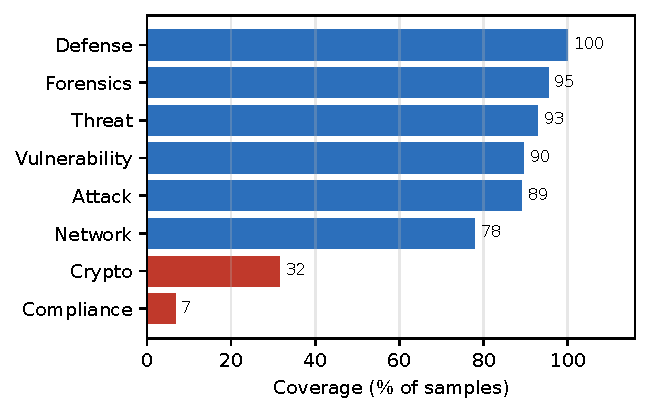
\includegraphics[width=\columnwidth]{fig_domains.pdf}
  \caption{Domain coverage of the defensive dataset. Compliance
  (highlighted) is the dominant coverage gap.}
  \label{fig:domains}
\end{figure}

\subsection{Offensive exploitation dataset}

The offensive branch (\offensivename) departs from the defensive pipeline in
purpose and in method. It takes the public
\texttt{CyberNative/\allowbreak Code\_\allowbreak Vulnerability\_\allowbreak Security\_\allowbreak DPO}
corpus~\cite{cybernative} and, for each vulnerable code sample, uses an
abliterated local model to synthesize an assistant answer that
identifies the vulnerability and provides exploitation guidance,
structured as an audit summary, findings, exploitation steps, and payload
examples. Table~\ref{tab:offensive-sizes} gives the split sizes; a
metadata file records per-record provenance (source dataset, row index,
language, and vulnerability class).

% AUTO-GENERATED by gen_tables.py -- do not edit
\begin{table}[t]
\centering
\small
\caption{Offensive exploitation SFT dataset, synthesized by an abliterated model over the public CyberNative Code\_Vulnerability\_Security\_DPO corpus.}
\label{tab:offensive-sizes}
\begin{tabular}{lr}
\hline
\textbf{Split} & \textbf{Records} \\
\hline
Train & 4,656 \\
Validation & 465 \\
Test & 419 \\
\textbf{Total} & \textbf{5,540} \\
\hline
\end{tabular}
\end{table}


Two design choices make this branch the ethically load-bearing part of the
work: it \emph{omits} the security-alignment stage the defensive pipeline is
meant to include, and it uses a de-aligned generator so the synthesis does not
refuse. (\S\ref{sec:dualuse}).

\subsection{Preference data}

A third, defensive preference dataset is derived from the same CyberNative
source for DPO/ORPO training: the \emph{chosen} response is a safe rewrite of
the vulnerable code and the \emph{rejected} response retains the
vulnerability.

\section{Fine-Tuning Recipes}
\label{sec:recipes}

All fine-tuning uses low-rank adaptation on quantized open models under MLX on
a single Apple~Silicon machine. We train across four base models: Qwen3-30B-A3B
in both Instruct and Thinking variants (8-bit), a $120$B mixture-of-experts
model (\texttt{gpt-oss-120b}, 4-bit), and abliterated Qwen3
variants, covering the aligned/abliterated and defensive/offensive
combinations studied in \S\ref{sec:results}.

Table~\ref{tab:hyperparams} lists the two representative recipes read directly
from the released training configs: supervised LoRA instruction tuning, and
DPO preference tuning. The SFT recipe adapts the last $16$ layers with rank-$8$
adapters (scale $16$) across all attention and MLP projections at learning
rate $2\times10^{-4}$; the DPO recipe adapts all layers with a KL penalty
$\beta=0.1$ and an effective batch size of $8$. ORPO runs use rank-$16$
adapters (scale $32$). All runs use gradient checkpointing to fit within
memory and log to Weights~\&~Biases.

% AUTO-GENERATED by gen_tables.py -- do not edit
\begin{table}[t]
\centering
\small
\caption{Fine-tuning hyperparameters, read from the released training configs. SFT column: LoRA instruction tuning; DPO column: preference tuning.}
\label{tab:hyperparams}
\begin{tabular}{lrr}
\hline
\textbf{Parameter} & \textbf{SFT} & \textbf{DPO} \\
\hline
Fine-tune type & lora & dpo \\
LoRA rank & 8 & 8 \\
LoRA scale & 16.0 & 10.0 \\
LoRA dropout & 0.05 & 0.05 \\
Layers tuned & 16 & all \\
Batch size & 2 & 2 \\
Grad accumulation & -- & 4 \\
Learning rate & 2e-4 & 2e-4 \\
Iterations & 1416 & 200 \\
Max seq length & 4096 & 2048 \\
Optimizer & adamw & adamw \\
DPO $\beta$ & -- & 0.1 \\
Seed & 42 & -- \\
\hline
\end{tabular}
\end{table}


\section{Training Dynamics and Cost}
\label{sec:results}

We logged training telemetry to Weights~\&~Biases for the fine-tuning runs:
train and validation loss, throughput, and peak memory. The capability and safety of the resulting models
are measured separately in \S\ref{sec:eval}. Fifteen runs have usable
histories; Table~\ref{tab:training-runs} lists
representative runs.

% AUTO-GENERATED by gen_wandb.py -- do not edit
\begin{table*}[t]
\centering
\caption{Representative LoRA runs from training telemetry. These are \emph{training} metrics only; no capability or safety evaluation was logged. `min' is the best validation loss reached.}
\label{tab:training-runs}
\footnotesize
\setlength{\tabcolsep}{5pt}
\begin{tabular}{llllrrr}
\hline
\textbf{Base model} & \textbf{Align.} & \textbf{Data} & \textbf{State} & \textbf{Steps} & \textbf{Train loss} & \textbf{Val loss (min)} \\
\hline
Qwen3-30B Instruct (8b) & aligned & defensive (instruction) & finished & 142 & 0.994$\to$0.613 & 1.268$\to$0.553 (0.548) \\
Qwen3-30B Instruct (8b) & aligned & defensive (instruction) & finished & 142 & 1.014$\to$0.617 & 1.313$\to$0.552 (0.548) \\
Qwen3-30B Instruct (8b) & abliterated & defensive (instruction) & finished & 142 & 1.133$\to$0.584 & 1.517$\to$0.492 (0.489) \\
Qwen3-30B Instruct (8b) & aligned & offensive (Code\_Vulns) & finished & 466 & 1.066$\to$0.299 & 2.665$\to$0.301 (0.248) \\
Qwen3-30B Instruct (8b) & abliterated & offensive (Code\_Vulns) & finished & 466 & 1.175$\to$2.018 & 2.853$\to$4.451 (0.228) \\
gpt-oss-120b (4-bit) & aligned & defensive (instruction) & killed & 31 & 2.76$\to$1.095 & 8.959$\to$0.954 (0.954) \\
Qwen3-4B Instruct & abliterated & offensive (Code\_Vulns) & finished & 233 & 1.448$\to$0.367 & 1.564$\to$0.354 (0.354) \\
Qwen3-4B Instruct & abliterated & offensive (Code\_Vulns) & killed & 336 & 0.88$\to$3.104 & 1.524$\to$3.086 (0.57) \\
\hline
\end{tabular}
\end{table*}


\paragraph{Convergence.}
On the defensive instruction data, the aligned Qwen3-30B Instruct model
converges smoothly to a best validation loss of $0.548$, and the offensive
Code\_Vulns objective on the same base reaches a lower best validation loss of
$0.248$ (Figure~\ref{fig:loss-dataset}), which is not surprising, as the offensive
targets are longer, more templated, and less varied than the diverse
defensive corpus. Lower loss here reflects easier fitting, not a safety or
capability claim.

\begin{figure}[t]
  \centering
  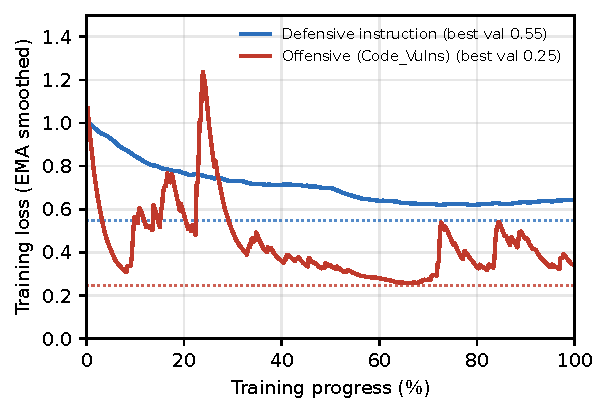
\includegraphics[width=\columnwidth]{fig_loss_dataset.pdf}
  \caption{Training loss (EMA smoothed) versus training progress on Qwen3-30B
  Instruct: defensive instruction data versus the offensive Code\_Vulns
  objective. The offensive
  objective fits to a lower loss.}
  \label{fig:loss-dataset}
\end{figure}

\paragraph{Aligned versus abliterated.}
Holding the data fixed (the formatted defensive set), the abliterated
Qwen3-30B base reaches a best validation loss of $0.489$, slightly below the
aligned Instruct model's $0.548$ (Figure~\ref{fig:loss-alignment}). Removing
refusal behavior does not impede (and marginally eases) fitting the
cybersecurity data. A de-aligned base is at least as amenable to this
fine-tuning as its aligned counterpart.

\begin{figure}[t]
  \centering
  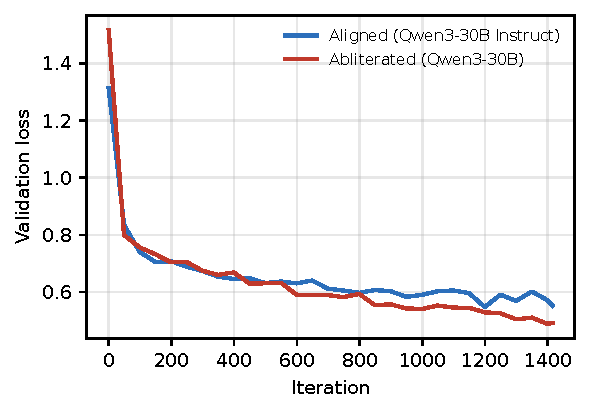
\includegraphics[width=\columnwidth]{fig_loss_alignment.pdf}
  \caption{Validation loss on identical defensive data: aligned versus
  abliterated Qwen3-30B. De-alignment does not hurt convergence.}
  \label{fig:loss-alignment}
\end{figure}

\paragraph{Training instability.}
Several offensive and abliterated runs did not converge cleanly. The
abliterated Qwen3-30B on Code\_Vulns diverged (validation loss rising from
$2.853$ to $4.451$), and an abliterated Qwen3-4B run destabilized late
(validation loss $1.524\to3.086$). These indicate that the offensive/de-aligned
configuration is more sensitive to schedule and length than the defensive one.

\paragraph{Cost on consumer hardware.}
The cost that matters to an adversary is wall clock time on owned hardware, not
the streaming rate. A complete offensive fine-tune of the 30B model finished in
$6.5$~hours over $8.0$~million tokens on a single Apple~Silicon machine; the 4B
model, run to a longer schedule, took up to $18.6$~hours and $25.2$~million
tokens (wall clock here tracks the iteration budget, not model size). Throughput
was $275$--$740$ tokens per second within $34.6$--$79.1$\,GB of memory
(Table~\ref{tab:training-cost}); the $120$B model was the slowest and most
memory-hungry, at about $275$ tokens per second and $79.1$\,GB. There is no
cloud bill and no costs beyond hardware and electricity: one desktop left running for
an afternoon or overnight is the entire capital requirement.

% AUTO-GENERATED by gen_wandb.py -- do not edit
\begin{table}[t]
\centering
\caption{LoRA fine-tuning throughput and peak memory on a single Apple~Silicon machine. Ranges span the usable runs for each base model.}
\label{tab:training-cost}
\small
\setlength{\tabcolsep}{3pt}
\begin{tabular}{lrr}
\hline
\textbf{Base model} & \textbf{Tok/s} & \textbf{Peak (GB)} \\
\hline
Qwen3-4B Instruct & 468--568 & 34.6 \\
gpt-oss-120b (4-bit) & 275--309 & 79.1 \\
Qwen3-30B Thinking (8b) & 509--739 & 35.2--35.3 \\
Qwen3-30B Instruct (8b) & 404--641 & 35.5--76.2 \\
\hline
\end{tabular}
\end{table}


\section{Measured Capability/Safety Evaluation}
\label{sec:eval}

Beyond training dynamics (\S\ref{sec:results}), we evaluate the models
themselves along two axes that jointly define the dual-use question:
\emph{alignment} (an aligned base vs.\ its abliterated counterpart) and
\emph{fine-tuning} (the base vs.\ the same base offensively fine-tuned on
\offensivename). Every cell is measured on three suites.

We train a LoRA adapter for each base on the offensive data, following the recipe of \S\ref{sec:recipes}, at learning rate $1\times10^{-4}$ for the aligned bases and $5\times10^{-5}$ for the abliterated ones.

\paragraph{Capability.}
Cybersecurity knowledge is scored with CyberMetric-500~\cite{cybermetric}, a
human-validated four option multiple-choice benchmark, as exact match accuracy.

\paragraph{Safety.}
We measure two rates over the held out exploit request set. The
\emph{refusal rate} is the fraction of requests the model declines; the
\emph{attack-success rate} (ASR) is the fraction for which it returns concrete,
actionable exploitation content. To isolate the model's own alignment from any
prompt level jailbreak, the exploitation ask is issued under a \emph{neutral}
system prompt rather than the dataset's red team system prompt, so the measured
refusal reflects the model (and adapter), not the framing.

\paragraph{Quality.}
Under the dataset's intended use audit prompt, a judge scores each audit answer
against the ground truth reference on a $1$--$5$ correctness and format rubric.

\paragraph{Judge.}
Safety labeling and quality scoring use an abliterated judge model, a
deliberate choice: a safety-aligned judge would itself refuse to read and score
exploitation content, corrupting exactly the measurements we need. The judge is
a scorer, not a subject under test; we flag this as a validity caveat, and note
that judge labels were spot-checked by hand.

We evaluate six base models: Qwen3-4B, Qwen3-30B-A3B, and gpt-oss-20B, each in
an aligned and an abliterated variant, as-is and after offensive fine-tuning,
for twelve configurations in total (Table~\ref{tab:eval-matrix}). CyberMetric
runs over all 500 questions; the safety and quality suites use 150 held out
exploit requests each, scored by the judge.

% Results table generated by eval/aggregate.py -> eval/results/results.tex.
% AUTO-GENERATED by eval/aggregate.py -- do not edit
\begin{table*}[t]
\centering
\small
\caption{Capability--safety evaluation matrix. Capability is CyberMetric-500 accuracy (\%); safety is refusal rate and attack-success rate (ASR, \%) on held out exploit requests; quality is the abliterated-judge audit score (1--5). For each base model we report the model as-is and after offensive fine-tuning (ft). Higher accuracy/quality and higher refusal are safer directions; higher ASR is more dangerous. $^{\dagger}$ computed over valid generations (25.3\% generation-failure rate, see text).}
\label{tab:eval-matrix}
\begin{tabular}{llcccc}
\hline
\textbf{Model} & \textbf{Align.} & \textbf{CyberMetric} & \textbf{Refusal} & \textbf{ASR} & \textbf{Quality} \\
\hline
Qwen3-4B & aligned & 89.0 & 22.7 & 63.3 & 3.84 \\
 & aligned +ft & 90.2 & 0.0 & 96.0 & 4.19 \\
\hline
Qwen3-4B & abliterated & 88.2 & 0.0 & 92.0 & 3.95 \\
 & abliterated +ft & 88.6 & 0.0$^{\dagger}$ & 92.9 & 4.18 \\
\hline
Qwen3-30B & aligned & 93.6 & 1.3 & 93.3 & 4.42 \\
 & aligned +ft & 93.0 & 0.0 & 100.0 & 4.62 \\
\hline
Qwen3-30B & abliterated & 91.4 & 0.0 & 100.0 & 4.75 \\
 & abliterated +ft & 91.4 & 0.0 & 99.3 & 4.72 \\
\hline
gpt-oss-20B & aligned & 91.8 & 23.3 & 71.3 & 4.16 \\
 & aligned +ft & 85.8 & 0.0 & 98.0 & 4.61 \\
\hline
gpt-oss-20B & abliterated & 88.6 & 0.0 & 98.0 & 4.06 \\
 & abliterated +ft & 78.6 & 0.0 & 98.7 & 4.52 \\
\hline
\end{tabular}
\end{table*}


\paragraph{Abliteration is nearly capability free.}
Across all three model families, removing refusals costs little cyber knowledge:
CyberMetric moves by at most a few points between an aligned base and its
abliterated counterpart (e.g.\ Qwen3-4B $89.0\to88.2$, Qwen3-30B
$93.6\to91.4$). Yet the same abliteration collapses refusal to near zero and
pushes ASR toward saturation. Un-aligning a capable security model is, in
capability terms, almost free.

\paragraph{Alignment is thin against security framing, and family dependent.}
The aligned bases differ sharply in how much they refuse the (neutrally framed)
exploit requests: Qwen3-30B-aligned refuses only $1.3\%$ despite being the most
capable model in the study, whereas the smaller Qwen3-4B-aligned refuses
$22.7\%$ and gpt-oss-20B-aligned $23.3\%$. Refusal therefore does not simply
track capability; gpt-oss retains meaningful alignment at a capability
($91.8$) comparable to Qwen3-30B's, so the erosion is a property of the model's
safety training, not of scale alone.

\paragraph{Offensive fine-tuning strips alignment on every base.}
This is the central result. Fine-tuning drives refusal to $0\%$ and ASR to
$96$--$100\%$ for \emph{every} configuration, including the two that retained
real refusal: Qwen3-4B-aligned ($22.7\%\to0\%$ refusal, $63.3\to96.0$ ASR) and
gpt-oss-20B-aligned ($23.3\%\to0\%$, $71.3\to98.0$). Abliteration is one route
to a refusal-free security model; offensive fine-tuning is an independent one
that reaches the same endpoint from an aligned start, and audit quality
\emph{rises} throughout (every ft row scores higher than its base).

\paragraph{Fine-tuning taxes gpt-oss capability but not Qwen.}
The one axis on which the families diverge is capability retention under
fine-tuning. Qwen barely moves (Qwen3-4B $89.0\to90.2$, Qwen3-30B
$93.6\to93.0$), but gpt-oss loses ground: $91.8\to85.8$ (aligned) and
$88.6\to78.6$ (abliterated). Offensive fine-tuning is not uniformly free: on
gpt-oss it trades measurable capability for the removal of refusals.

\paragraph{Fine-tuning an abliterated base is unstable.}
The Qwen3-4B abliterated model, fine-tuned on the offensive data, produced
degenerate generations (empty output or special-token loops) on $25.3\%$ of
inputs even after lowering the learning rate; we exclude those from the rates
and report the failure directly (Table~\ref{tab:eval-matrix}, $\dagger$). The
30B abliterated model was stable, so this is a small model fragility rather than
a general one, but it means stacking fine-tuning on an already-de-aligned base
is the least reliable path, not a strictly stronger one.

\section{Dual-Use Analysis and Broader Impacts}
\label{sec:dualuse}

None of the individual steps above is novel; their cheap combination, and its
implication, is the point of the paper. Every ingredient needed to produce a
locally hosted, exploitation oriented security model is now freely available and
cheap to combine: authoritative sources, a public vulnerable code
corpus~\cite{cybernative}, open abliterated models~\cite{abliteration}, and an
on-device training stack (\S\ref{sec:results}). No cloud provider, and therefore
no safety moderation, sits anywhere in this loop.

\paragraph{Threat model.}
The actor we have in mind is not slamming rate-limits, but analyzing vulnerabilities offline.
They do not need an API budget, data sharing agreement, and any moderation filter to
evade. As \S\ref{sec:results} and \S\ref{sec:datasets} show, the barrier is low:
de-alignment does not impair fitting the security data, the offensive objective
is in fact \emph{easier} to fit than the defensive one, and the offensive branch
simply omits the safety-alignment stage that the defensive pipeline includes.

\paragraph{Threat intelligence implications.}
Our measurements (\S\ref{sec:eval}) point to a
threat intelligence conclusion: the realistic near-term offensive LLM threat is
\emph{offline and uncensored}, and therefore more difficult for the
detection surfaces most defenders rely on. Three factors compound. First,
because the whole loop is local, no provider side telemetry or abuse signal is
ever generated; there is no API to monitor. Second, because
abliteration is capability-free (\S\ref{sec:eval}), an adversary obtains a fully
capable LLM without any fine-tuning skills. Third, exploitation
requests framed as ordinary code audits do not resemble jailbreaks, so
prompt level signatures miss them. The defensive takeaway is to expect less
API level or jailbreak signature detection to catch this class of tool and to
shift toward endpoint, output-artifact, and open source signals. For example the
characteristic audit/exploit output structure and the public
fingerprints of the training data. Adversary infrastructure is not the barrier, but
\emph{knowledge} (which weights to download and which tool to run), and that
knowledge is public and social. The useful collection surface is the
distribution layer, not the local inference: abliteration tooling
repositories, the model hubs that host de-aligned outputs, and the forums that
circulate configurations and setups are cheaper to watch and carry earlier
signal. The \emph{marginal} uplift of offensive
fine-tuning over simply using an abliterated base (\S\ref{sec:eval}) is itself a
triage signal: a small delta means the abliterated base is the threat and
bespoke fine-tunes do not need to be tracked separately, while a large delta marks
custom offensive fine-tuning as a distinct escalation. In our matrix this delta
is small: abliterated bases are already uncensored and
near saturated on attack-success (Table~\ref{tab:eval-matrix}), so the
abliterated base itself is the operative threat.

% AUTO-GENERATED by eval/calc_hardware.py -- do not edit
\begin{table*}[t]
\centering
\small
\caption{Inference hardware floor. Memory footprint is computed (weights at the listed quantization $+$ an 8k-token KV cache $+$ runtime overhead) and matches published GGUF sizes. `Active' is the parameters computed per token, which for the mixture-of-experts models is far below the resident total, so the 30B-class model runs at interactive speed on a CPU. Costs are approximate US used/consumer prices surveyed in August~2026 for the cheapest sufficient hardware; the 2026 AI-driven memory and GPU shortage has raised them from earlier lows, yet the floor stays within a few hundred dollars.}
\label{tab:hardware-floor}
\setlength{\tabcolsep}{4pt}
\begin{tabular}{lrrll}
\hline
\textbf{Model} & \textbf{Mem} & \textbf{Active} & \textbf{Cheapest hardware} & \textbf{Cost} \\
\hline
Qwen3-4B (dense) & 3.7\,GB & 4.0\,B & any 8\,GB laptop/PC, CPU & owned / \$0 \\
gpt-oss-20B (MoE) & 12.2\,GB & 3.6\,B & used 16\,GB GPU or 16\,GB PC & $\approx$\$550 \\
Qwen3-30B-A3B (MoE) & 19.5\,GB & 3.3\,B & 32\,GB mini-PC (CPU) or used 24\,GB GPU & \$650--800 \\
\hline
\end{tabular}
\end{table*}


\paragraph{Hardware floor.}
Our experiments ran on an Apple~M4~Max with $128$\,GB of unified memory, but
that overstates the requirement: the threat action is \emph{inference} of an
abliterated base, and inference is memory-bound. Table~\ref{tab:hardware-floor}
gives each model's computed footprint at standard GGUF quantization. The $4$B
model fits in under $4$\,GB, within reach of any laptop of the last decade, yet still scores $88.2$ on CyberMetric with refusals removed. The
mixture-of-experts models are the sharper case: they keep $20$--$30$B
parameters resident but compute only ${\sim}3.3$B per token, so the most
capable model in the study ($93.6$ on CyberMetric) runs at interactive speed on
a commodity $32$\,GB mini-PC with no GPU (roughly \$550 as a complete machine in
mid-2026) or a used $24$\,GB card (an RTX~3090 around \$700), and hardware many
operators already own costs nothing further. That floor has in fact risen over $2026$: the same AI demand this paper studies
drove a memory and GPU shortage that roughly doubled these prices.

\paragraph{What we withhold, and why.}
Consistent with responsible disclosure norms for dual-use security research, we
report enough to substantiate the risk and no more:
\begin{itemize}
  \item We do \emph{not} release the offensive dataset, its exploit content, or
  any example payloads. It is characterized only by size and provenance
  (\S\ref{sec:datasets}).
  \item We do \emph{not} release offensive adapter weights or fused models.
  \item We report only \emph{aggregate} capability and safety metrics
  (\S\ref{sec:eval}); we do not release the per-example generations behind
  them, an offensive utility scorecard, or any runnable tool.
  \item The upstream sources we name are already public; we add no new
  offensive capability, only a measurement of how cheaply existing pieces
  compose.
\end{itemize}

\paragraph{Significance.}
The safety/performance trade-off in cybersecurity fine-tuning is already
documented~\cite{cyberllminstruct,qi2023finetuning,lermen2023lora}; what is new
is that it can now be realized entirely offline, at negligible cost, on a
de-aligned base. Defenders, model distributors, and hardware/software vendors
benefit from knowing this: it argues for treating abliterated model
distribution, forums, and local fine-tuning as part of the threat surface.

\section{Limitations}
\label{sec:limitations}

\paragraph{Evaluation validity caveats.}
The abliterated models are community builds whose quantization
differs from their aligned counterparts, so a small part of any aligned versus abliterated capability gap may be quantization rather than abliteration. The
judge is a single abliterated model, not a human panel; we spot-checked its
labels but did not measure inter-rater agreement. The Qwen3-4B abliterated fine-tune was unstable
($25.3\%$ generation failures, excluded from its rates), which both narrows its
effective sample and signals that that particular cell is the least reliable in
the matrix.

\paragraph{Measurement caveats.}
Domain coverage is computed by overlapping keyword matching and so should be
read as coarse. Throughput and memory figures come from a single machine and a
small number of runs; several runs were killed or crashed, and this run set is
not a controlled sweep. The aligned versus abliterated comparison holds
the data fixed but varies only two runs, so it is indicative rather than
statistically established.

\paragraph{Artifacts not released.}
Beyond the offensive artifacts withheld in \S\ref{sec:dualuse}, the defensive
dataset is also not released. This
limits direct reproducibility of the data, a tension we accept in exchange for
not distributing artifacts.

\section{Conclusion}
\label{sec:conclusion}

We reimplemented a published cybersecurity instruction data pipeline to run
entirely on a local machine, removing every external service
from the construction and fine-tuning loop, and we used the same
infrastructure to build an offensive branch that removes safety alignment and
trains on exploitation data over several model bases. Measuring a full
alignment~$\times$~fine-tuning matrix across three model families, we found
abliteration and offensive fine-tuning to be two cheap routes to a
refusal free, capable model, with a complete fine-tune finishing in hours on
commodity hardware only costing electricity. The contribution is a
measured insight: the pieces required to build a locally hosted, exploitation
AI model are public, cheap, and offline, and the safety guardrails that a
cloud pathway would impose are absent by design. Treating local
fine-tuning, abliterated model distribution, and configuration forums as first class parts of the
threat surface is the appropriate response.


\bibliographystyle{plain}
\bibliography{references}

\end{document}
